\documentclass[xetex,mathserif,serif]{beamer}
\usepackage{graphicx}
\usepackage{amsmath}
\usepackage{tikz}
\usetikzlibrary{automata, positioning}

\DeclareMathOperator*{\argmax}{argmax}
\DeclareMathOperator*{\argmin}{argmin}

\title {Multitarget List Viterbi Tracking Algorithm}
\author {Tom Boyd}
\institute[SciTec] % (optional)
{
  SciTec Inc.\\
  100 Wall Street\\
  Princeton, NJ 08540
}
\date{\today}

\begin{document}
\frame{\titlepage}

\begin{frame}{Hidden Markov Models}
    \begin{itemize}
        \item Discrete-time, countable-state Markov process observed in
              memoryless noise
        \item Nothing is a deterministic function of state sequence
        \item Dependence is only between adjacent states and direct
              observations with their associated states.
        \item Probability of “transition” and probabilities of observation
        \item Represented by simplest dynamic Bayesian network
    \end{itemize}

    \begin{figure}
        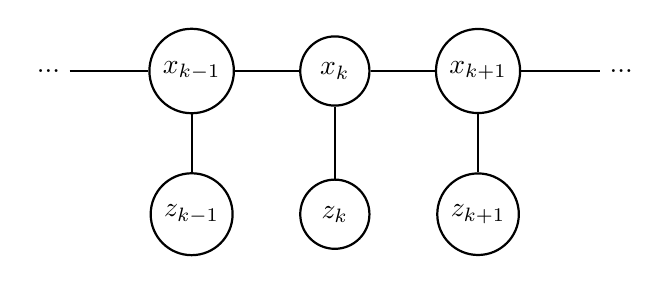
\begin{tikzpicture}[node distance=.15\textwidth]
    \node (begin) {...};
    \node[state, thick] (xk-1)[right of=begin] {$x_{k-1}$};
    \node[state, thick] (xk)[right of=xk-1]    {$x_k$};
    \node[state, thick] (xk+1)[right of=xk]    {$x_{k+1}$};
    \node[state, thick] (zk-1)[below of=xk-1]  {$z_{k-1}$};
    \node[state, thick] (zk)[below of=xk]      {$z_k$};
    \node[state, thick] (zk+1)[below of=xk+1]  {$z_{k+1}$};
    \node (end)[right of=xk+1] {...};
    \draw[thick]
        (begin)   edge node {} (xk-1)
        (xk-1)    edge node {} (xk)
        (xk)      edge node {} (xk+1)
        (xk+1)    edge node {} (end)
        (zk-1)    edge node {} (xk-1)
        (zk)      edge node {} (xk)
        (zk+1)    edge node {} (xk+1);

\end{tikzpicture}

        \caption{HMM dependence graph: lines represent dependence}
    \end{figure}
\end{frame}

\begin{frame}{Hidden Markov Model Parameters and Properties}
    \begin{itemize}
    \item A Hidden Markov model is parameterized by the following Parameters
    \begin{description}[Test]
        \item[$M$] Cardinality of state space.
        \item[$T$] Cardinality of observation space.
        \item[$A$] State transition matrix $(M \times M)$:
            $a_{i,j} \triangleq P(x_{k+1} = j | x_k = i)$
        \item[$B$] Emission matrix $ (M \times T)$:
            $b_{i,j} \triangleq P(z_k = j | x_k = i)$
        \item[$\boldsymbol \pi$] initial state probabilities:
            $\pi_i \triangleq P(x_0 = i)$
    \end{description}

    \item Associated with the model are the following processes:
    \begin{description}[test]
        \item[$\mathbf x$] state sequence:
            $\mathbf x = (x_0, x_1, \ldots, x_K)$
        \item[$\mathbf z$] observation sequence:
            $\mathbf z = (z_0, z_1, \ldots, z_K)$
    \end{description}

    \item Obviously, Markov Property holds:
    \begin{equation}
        P(x_k | x_{k-1}, \ldots, x_0) = P(x_k | x_{k-1})
    \end{equation}
    \end{itemize}
\end{frame}

\begin{frame}{HMM Diagrams}
    \begin{columns}[c] % the "c" option specifies center vertical alignment
        \column{.5\textwidth} % column designated by a command
        \begin{figure}
            \resizebox {\columnwidth} {!} {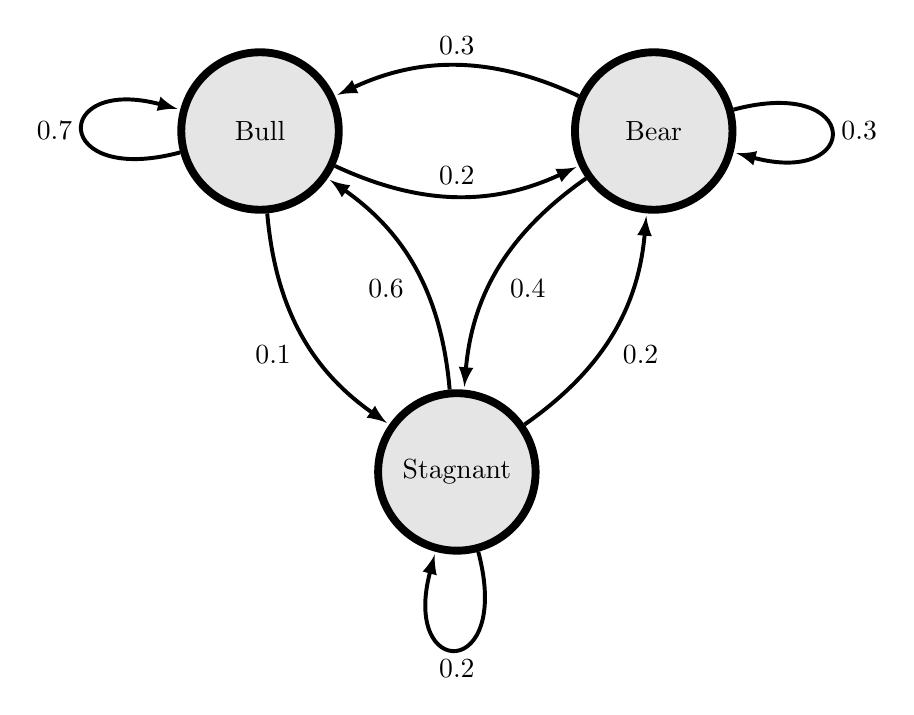
\begin{tikzpicture}
    % Setup the style for the states
    \tikzset{node style/.style={state,
                                minimum width=2cm,
                                line width=1mm,
                                fill=gray!20!white}}

    % Draw the states
    \node[node style] at (0, 0)       (bull)     {Bull};
    \node[node style] at (5, 0)       (bear)     {Bear};
    \node[node style] at (2.5, -4.33) (stagnant) {Stagnant};

    % Connect the states with arrows
    \draw[every loop, auto=right, line width=.5mm, >=latex]
        (bull)     edge[bend right=25]            node {0.1} (stagnant)
        (bull)     edge[bend right=25, auto=left] node {0.2} (bear)
        (bear)     edge[bend right=25]            node {0.3} (bull)
        (bear)     edge[bend right=25, auto=left] node {0.4} (stagnant)
        (stagnant) edge[bend right=25]            node {0.2} (bear)
        (stagnant) edge[bend right=25, auto=left] node {0.6} (bull)
        (stagnant) edge[loop below]               node {0.2} (stagnant)
        (bull)     edge[loop left]                node {0.7} (bull)
        (bear)     edge[loop right]               node {0.3} (bear);
\end{tikzpicture}
}
            \caption{State diagram: digraph representation of Markov chain}
        \end{figure}

        \column{.5\textwidth}
        \begin{figure}
            \resizebox {\columnwidth} {!}{ 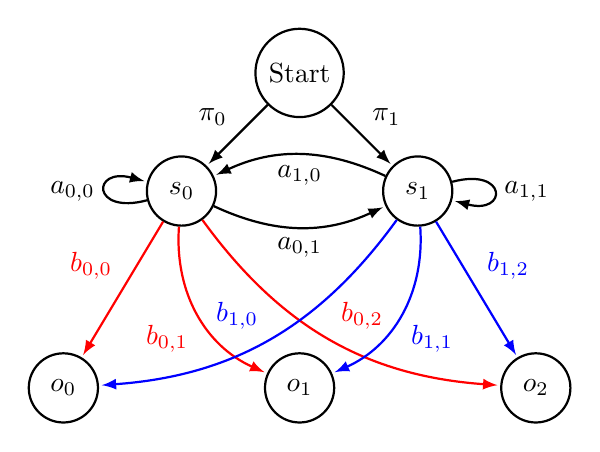
\begin{tikzpicture}
    \node[state, thick] (start) at (0, 0) {Start};
    \node[state, thick] (x0) at (-1.5, -1.5) {$s_0$};
    \node[state, thick] (x1) at (1.5, -1.5) {$s_1$};
    \node[state, thick] (z0) at (-3, -4) {$o_0$};
    \node[state, thick] (z1) at (0, -4) {$o_1$};
    \node[state, thick] (z2) at (3, -4) {$o_2$};

    \draw[every loop, >=latex, auto=right, thick]
        (start) edge node {$\pi_0$} (x0)
        (start) edge[auto=left] node {$\pi_1$} (x1)
        (x0) edge[bend right=25, auto=right]      node {$a_{0,1}$} (x1)
        (x1) edge[bend right=25, auto=left]       node {$a_{1,0}$} (x0)
        (x0) edge[loop left]                      node {$a_{0,0}$} (x0)
        (x1) edge[loop right]                     node {$a_{1,1}$} (x1)
        (x0) edge[red]                            node {$b_{0,0}$} (z0)
        (x0) edge[bend right=35, auto=right, red] node {$b_{0,1}$} (z1)
        (x0) edge[bend right=25, auto=left, red]  node {$b_{0,2}$} (z2)
        (x1) edge[bend left=25, blue]             node {$b_{1,0}$} (z0)
        (x1) edge[bend left=35, auto=left, blue]  node {$b_{1,1}$} (z1)
        (x1) edge[auto=left, blue]                node {$b_{1,2}$} (z2);
\end{tikzpicture}
 }
            \caption{Hidden Markov Model state diagram}
        \end{figure}
    \end{columns}
    \begin{itemize}
        \item State diagrams consisting of digraphs: Nodes representing states
              and edges representing transitions.
        \item Edges labeled with transition probabilities
    \end{itemize}
\end{frame}

\begin{frame}{Viterbi Algorithm Overview}
    \begin{itemize}
    \item Maximum a posteriori Probability Estimator of HMM state sequence:
          $\argmax_{\mathbf x} P(\mathbf x | \mathbf z)$
    \item Recursive dynamic programming algorithm
    \item Exploits Markov property to make polynomial time solution to problem
          with factorial time marginalization methods.
    \item Most commonly used in convolutional decoders. Still used in CDMA,
          GSM modems, satellite, deep-space, and 802.11
    \item Also commonly used in speech recognition, speech synthesis,
          diarization, computational linguistics, and bioinformatics
    \end{itemize}
\end{frame}

\begin{frame}{Viterbi Algorithm Background}
    \begin{itemize}
    \item Assume process runs from time 0 to $K$ and states $x_0$ and $x_K$ are
          known. It is shown trivial to extend to infinite sequences.
    \item Define transitions at time $k$ and transition sequence:
    \begin{equation}
    \begin{aligned}
    \xi_k &\triangleq (x_k, x_{k+1})\\
    \boldsymbol \xi &= (\xi_0, \ldots, \xi_{K-1}) \leftrightarrow \mathbf x
    \end{aligned}
    \end{equation}
    \item Due to memoryless noise channel, $z_k$ depends only on $\xi_k$:
    \begin{equation}
        P(\mathbf z | \mathbf x) = P(\mathbf z | \boldsymbol \xi) =
        \prod_{k=0}^{K-1} P(z_k | \xi_k)
    \end{equation}
    \item Viterbi algorithm is a recursive solution to
    \begin{equation}
        \mathbf{\hat x} = \argmax_{\mathbf x} P(\mathbf x | \mathbf z)
    \end{equation}
    \end{itemize}
\end{frame}

\begin{frame}{Trellis Structure}
    \begin{itemize}
    \item Trellis structure introduced to frame recursive optimization solution
    \item In general, $P(z_k | x_k)$ depends on $k$, allowing assumption of
          $x_K$ and $x_0$
    \item Trellis nodes represent a distinct state at a given time ($x_k$),
          edges represent a transition to some new state ($\xi_k$)
    \end{itemize}
    \begin{figure}
        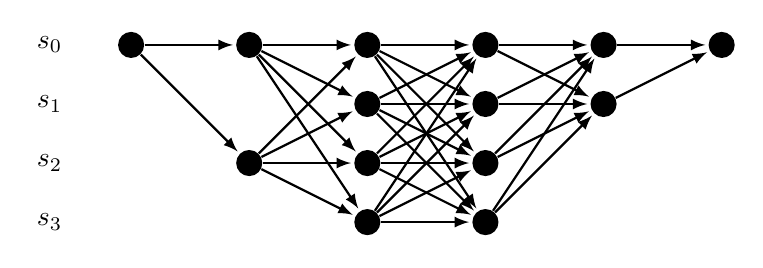
\begin{tikzpicture}[x=1.5cm, y=-.75cm]
    \node at (-0.5,0) [left] {$s_0$};
    \node at (-0.5,1) [left] {$s_1$};
    \node at (-0.5,2) [left] {$s_2$};
    \node at (-0.5,3) [left] {$s_3$};

    % Nodes
    \node (s00) at (0, 0)[circle, fill=black] {};
    \node (s10) at (1, 0)[circle, fill=black] {};
    \node (s12) at (1, 2)[circle, fill=black] {};
    \node (s20) at (2, 0)[circle, fill=black] {};
    \node (s21) at (2, 1)[circle, fill=black] {};
    \node (s22) at (2, 2)[circle, fill=black] {};
    \node (s23) at (2, 3)[circle, fill=black] {};
    \node (s30) at (3, 0)[circle, fill=black] {};
    \node (s31) at (3, 1)[circle, fill=black] {};
    \node (s32) at (3, 2)[circle, fill=black] {};
    \node (s33) at (3, 3)[circle, fill=black] {};
    \node (s40) at (4, 0)[circle, fill=black] {};
    \node (s41) at (4, 1)[circle, fill=black] {};
    \node (s50) at (5, 0)[circle, fill=black] {};

    % edges
    \draw[every loop, >=latex, thick]
        (s00) edge node {} (s10)
        (s00) edge node {} (s12)
        (s12) edge node {} (s20)
        (s12) edge node {} (s21)
        (s12) edge node {} (s22)
        (s12) edge node {} (s23)
        (s10) edge node {} (s20)
        (s10) edge node {} (s21)
        (s10) edge node {} (s22)
        (s10) edge node {} (s23)
        (s20) edge node {} (s30)
        (s20) edge node {} (s31)
        (s20) edge node {} (s32)
        (s20) edge node {} (s33)
        (s21) edge node {} (s30)
        (s21) edge node {} (s31)
        (s21) edge node {} (s32)
        (s21) edge node {} (s33)
        (s22) edge node {} (s30)
        (s22) edge node {} (s31)
        (s22) edge node {} (s32)
        (s22) edge node {} (s33)
        (s23) edge node {} (s30)
        (s23) edge node {} (s31)
        (s23) edge node {} (s32)
        (s23) edge node {} (s33)
        (s30) edge node {} (s40)
        (s30) edge node {} (s41)
        (s31) edge node {} (s40)
        (s31) edge node {} (s41)
        (s32) edge node {} (s40)
        (s32) edge node {} (s41)
        (s33) edge node {} (s40)
        (s33) edge node {} (s41)
        (s40) edge node {} (s50)
        (s41) edge node {} (s50);

\end{tikzpicture}

        \caption{Trellis Diagrams}
    \end{figure}
\end{frame}

\begin{frame}{Viterbi Solution}
    \begin{itemize}
    \item The MAP solution is formally equivalent to the minimum cost path
          (Viterbi path) through the trellis.
    \item Given $\mathbf z$, a cost function $\lambda(\mathbf x)$ is defined
        \begin{equation}
        \lambda(\mathbf x) \triangleq -\ln P(\mathbf x, \mathbf z)\,
        \forall\ \mathbf x : P(\mathbf x, \mathbf z) \ne 0
        \end{equation}

    \item Because paths are a bijection of state sequences, and $\ln$ is
          monotonically increasing, The Viterbi path is found by minimizing the
          cost function:
        \begin{equation}
            \begin{aligned}
            \argmax_{\mathbf x} P(\mathbf x | \mathbf z) &= \argmax_{\mathbf x}
            P(\mathbf x , \mathbf z)\\
            &= \argmin_{\mathbf x} \lambda(\mathbf x)
            \end{aligned}
        \end{equation}
    \end{itemize}
\end{frame}

\begin{frame}{Cost Function}
    \begin{itemize}
    \item Due to Markov property and memorylessness of channel noise, joint
          distribution factors as:
    \begin{equation}
    \begin{aligned}
    P(\mathbf x, \mathbf z) &= P(\mathbf x) P(\mathbf z | \mathbf x)\\
    &= \prod_{k=0}^{K-1} P(x_{k+1} | x_k) \prod_{k=0}^{K-1} P(z_k | \xi_k)
    \end{aligned}
    \end{equation}

    \item Assigning path cost function
    \begin{equation}
    \begin{aligned}
    \lambda(\xi_k) &\triangleq - \ln P(x_{k+1} | x_k) - \ln P(z_k | \xi_k)\\
    -\ln P(\mathbf x , \mathbf z) &= \sum_{k=0}^{K-1} \lambda(\xi_k)
    \end{aligned}
    \end{equation}
    \end{itemize}
\end{frame}

\begin{frame}{Viterbi Recursion}
    \begin{itemize}
    \item Let segment $\mathbf x_{0:k} \triangleq (x_0, \cdots x_k)$
    \item Cost function applies to segments.
    \begin{equation}
        \lambda(\mathbf x_{0:k}) = \sum_{i=0}^{k-1} \lambda(\xi_i)
    \end{equation}
    \item For every realization of $x_k$ there exists a minimum cost segment
        $\mathbf{\hat x}(x_k)$ called the \emph{survivor segment} for $x_k$.
    \begin{equation}
        \mathbf{\hat x}(x_k) = \argmin_{\mathbf x_{0:k}} \lambda(\mathbf x_{0:k})
    \end{equation}
    \item The complete Viterbi path, $\mathbf{\hat x}$, must begin with a
          survivor segment of one less time-length. (Proof by contradiction)
    \item Thus at any time $k$, the algorithm only needs to remember the $M$
          survivors $\mathbf{\hat x}(x_k)$ and their lengths
          $\lambda (\mathbf{\hat x}(x_k))$.
    \end{itemize}
\end{frame}

\begin{frame}{Formal statement of Viterbi algorithm}
    \begin{itemize}
    \item Define:
        \begin{equation}
            \Gamma(x_k) \triangleq \lambda(\mathbf{\hat x}(x_k))
        \end{equation}
    \item Initialize:
    \begin{equation}
        \begin{aligned}
            k &= 0\\
            \mathbf{\hat x}(x_0) &= x_0\\
            \Gamma(x_0) &= 0\\
        \end{aligned}
    \end{equation}
    \item Recursion:
        \begin{equation}
            \begin{aligned}
                \Gamma(x_{k+1}, x_k) &\triangleq \Gamma(x_k) + \lambda(\xi_k)\\
                \Gamma(x_{k+1}) &= \min_{x_k} \Gamma(x_{k+1}, x_k) \forall
                    x_{k+1}
            \end{aligned}
        \end{equation}
    \end{itemize}
\end{frame}

\begin{frame}{Practical Limitations}
    \begin{itemize}
        \item Typically, survivor segments all pass the same node at some time.
        \item Reclaim memory by truncating all survivor segments at
              $k - \delta$.
        \item For $\delta$ large enough, algorithm is still optimal with high
              probability.
        \item If $k$ becomes large, renormalize all costs by constant
              subtraction.
        \item Algorithm required to start with knowledge of $x_0$: Just assume
              it as initial state by definition.
    \end{itemize}
\end{frame}
\end{document}
